%zusammenfassung

%gegenseitige beeinflussung: showrooming-effekt: kauf online aufgrund von stationärere beratung -- kauf stationär nach onlinerecherche  \cite[S. 21f]{evilcom}

%wie viele läden haben in schleusingen einen onlineshop?


\begin{folding} %stationärer Handel

Aufgrund der Verschiebung von Nachfrage und Bedürfnissen von Konsumenten in den letzten Jahrzehnten wird der stationäre Handel trotz Multichannel-Versuchen keine einfache Zukunft haben. So kann in vielen Fällen stattdessen direkt von Herstellern gekauft werden, die mittlerweile den Vertriebswegwechsel von \ac{B2B} zu \ac{B2C} weitestgehend hinter sich haben. 
Insbesondere in Thüringen steht es im Vergleich zum Rest Deutschlands dank der Kombination aus schlechter Kaufkraft und niedriger Bevölkerungszahl pro Fläche schlecht um den konventionellen Einzelhandel \cite[S. 29]{Nitt}. Dazu kommen demografische Änderungen, die insbesondere in der Mitte Deutschlands Probleme verursachen: so nimmt die Bevölkerung z. B. in Hamburg, trotz Schrumpfen der Bevölkerungszahl, zu - jedoch nicht in Thüringen, eines der Bundesländer, welches am meisten Bewohner verliert \cite[S. 32f]{Nitt}. 
Zum Glück einiger Vertriebe treffen diese schlechten Chancen nicht auf alle Branchen zu - der Lebensmittelvertrieb hat z. B. kaum Online-Konkurrenz \cite{corona-schub}. Um in den restlichen Geschäftssektoren einen maximal großen Umsatz zu erzielen, sollte der konventionelle Einzelhandel aufgrund der alternden Bevölkerung, die meist noch stationär kauft, vorerst Investitionen für die wachsende Gruppe von Senioren und dementsprechend Erreichbarkeit o. ä. nutzen.

\end{folding}

\begin{folding} \subsubsection{Der Umwelt-Aspekt} %Umweltverschmutzung

Zudem kommt immer öfter das Argument auf, dass der Wechsel zum Onlinehandel umweltschädlich sei, da mehr Lieferfahrzeuge unterwegs sind. Jedoch haben bereits die Autoren des "Evil Commerce [...]"-Buches diese These anhand einer Modellrechnung weitestgehend widerlegt. Sie berechneten eine 89.1\%-ige Kraftstoffersparnis bei komplettem Umstieg zum Distanzhandel in Großstädten unter optimalen Bedingungen \cite[S. 25f]{evilcom}. Um genauerer Aussagen bezüglich des ländlichen Raumes zu treffen, werde ich die genannte Rechnung bzgl. Entfernung - da Einkaufszentren nicht berücksichtigt wurden - modifizieren und insofern erweitern, dass zusätzlich ein Einkauf in mehreren Geschäften nacheinander mit in Betracht gezogen wird.

\begin{itemize}

\item In meiner Modellrechnung kaufen 100 Bewohner eines Dorfes in einer 4km entfernten Stadt ein. Sie kaufen im Durchschnitt in 3 von 10 Einkaufsmöglichkeiten ein, die je 500m voneinander entfernt sind. Dabei gehe ich davon aus, dass alle Kunden über eine 500m lange Straße innerhalb des Dorfes zu erreichen sind.

\item Wenn alle Bewohner stationär kaufen, legen sie im Durchschnitt eine Strecke von 

\begin{align}(250m + 4000m + 3 \cdot 500m + 4000m + 250m) \cdot 100 = 1000000m\end{align}

 zurück. Dabei nehme ich an, dass alle Bewohner denselben Ortsausgang benutzen und somit einen durchschnittlichen Weg von 250m zu diesem besitzen.

\item Wenn jeder Verkäufer jedoch die Güter an seine im Durchschnitt 30 Kunden versendet, müssten alle Lieferwagen zusammen eine Strecke von gerade einmal 

\begin{align}(4000m + 500m + 4000m) \cdot 10 = 85000m\end{align}

zurücklegen.
\item In dieser Darstellung hat der Distanzhandel eine ähnlich hohe Kraftstoffersparnis - 91.5\%. 

\end{itemize}
Zwar kann mithilfe dieses Modelles die These der Umweltverschmutzung auch auf dem Land im Allgemeinen widerlegt werden, jedoch ist sie keine genaue Darstellung der Realität, da viele Faktoren, wie z. B. die Retouranzahl, die beispielsweise in der Modebranche überproportional hoch ist, nicht beachtet wurden (ebd.). Außerdem beschreibt diese Rechnung ein System der Güterbeschaffung, die ausschließlich über den Versandhandel stattfindet. Jedoch werden derzeit und in den nächsten Jahrzehnten aller Wahrscheinlichkeit nach Online- und Offlinehandel parallel benutzt werden - manche Produkte können nicht durch den Distanzhandel allein abgedeckt werden, zudem wird es immer Personen geben, die den analogen Beschaffungsweg bevorzugen und diesen somit wählen. Dementsprechend besteht trotzdem ein erhöhter Verbrauch. Bei einer annähernd vollständigen Umstellung auf den Distanzhandel  sind jedoch Kraftstoffersparnisse im Vergleich zu heute denkbar.

\end{folding}

\begin{folding} \subsubsection{Einfluss der Corona-Situation}
 % amazon gestärkt - einfluss auf kleine onlinehändler kaum spürbar
 
 Wie bereits in 4.1.2 angesprochen, schadet die Corona-Situation dem stationären Handel, insbesondere im Einzelhandelsbereich immens. Der Onlinehandel gewinnt aufgrund von flexibleren und bequemeren Verkaufsabläufen immer mehr Kunden, auch in Bereichen, die vom Offlinehandel dominiert werden, wie den \ac{FMCG}. 
Diese machten 2019 ohne Corona-Einfluss 42.5\% der stationären Verkäufe, und gleichzeitig nur 8.4\% der Verkäufe mittels Distanzhandel aus. Insgesamt wurden gerade einmal 2.2\% der \ac{FMCG} nicht vor Ort gekauft - jedoch ist diese Zahl im Verlauf von 2020 stark gestiegen \cite{corona-schub}. Insbesondere bei Produkten, die mit Corona in Verbindung gebracht werden können, steigt das Online-Interesse stark, wie man an folgender Auswertung von Google-Suchanfragen erkennen kann: 

 \begin{figure}[h]
    \begin{center}
        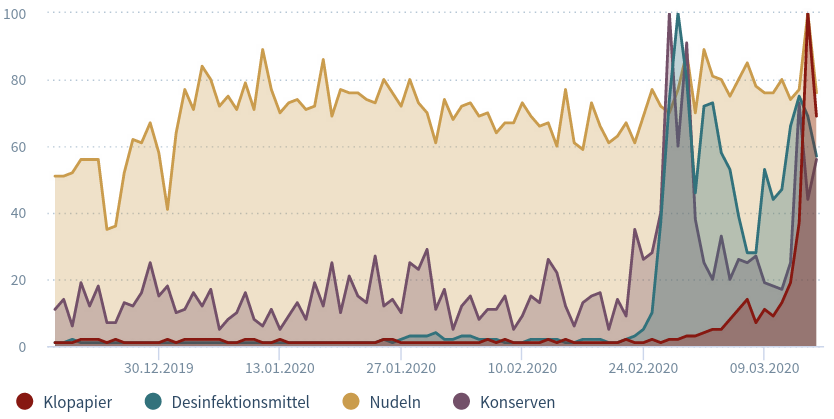
\includegraphics[width=8cm]{media/Fabian-Corona-Produkte.png}
        \caption{Onlinehandel: Die Deutschen im Krisenmodus}
        \label{corona-produkte}
        \bildquelle  Engels, Barbara:   Corona: Schub für den Onlinehandel. Version: 2020. https://bit.ly/38pdoqN. Köln: Institut der deutschen Wirtschaft (IW), 2020 (29/2020). – IW-Kurzbericht
    \end{center}
\end{figure}
\noindent Zudem ist es wahrscheinlich, dass

\begin{quote}
    "[...] Geschäftsschließungen und Ausgangsbeschränkungen   sowie Unsicherheiten über die Dauer der Maßnahmen zu einem  Nachfragerückgang [führen]." \cite{corona-wettbewerb}
\end{quote}
Des weiteren könnte die Angst, sich anzustecken ein weiterer Grund für den starken Nachfragezuwachs sein. Kunden, die vorerst ausschließlich stationär gekauft haben und nun erste Käufe online tätigen, können vor allem in Zukunft den Nachfrageumschwung von Offline- zu Onlinehandel noch verstärken \cite{corona-schub}. Dieser Trend machte sich auch bei unserer Schülerumfrage bemerkbar: 55 Schüler gaben an, dass sie mehr online kaufen als vor Corona-Zeiten - dagegen gab es nur eine Person, die mehr stationär kaufte als Anfang 2020. 92 Schülerinnen und Schüler bezeichneten ihre Kaufgewohnheiten als annähernd konstant(siehe Anhang, Frage 14).

%mehr zu stationär

Die immens hohe Nachfrage hat aber nicht ausschließlich positive Auswirkungen auf den Onlinehandel: eine Umfrage des Händlerbunds im März 2020 ergab, dass 52\% der befragten 412 Online-Unternehmen eine derart hohe Nachfrage erfuhren, dass diese zu Problemen führte - 15\% mussten sogar Aufträge stornieren. Als Grund sind logistische sowie personelle Probleme denkbar: So sind beispielsweise nicht immer Produktionsgüter verfügbar, da zurzeit die weltweiten Lieferketten eingeschränkt sind \cite{corona-wettbewerb}; zudem ist die Personalsituation je nach Branche und Gesetzgebung durch Corona-Regulationen eingeschränkt \cite{haendlerbund-studie}. Auch hier kann wie beim Einzelhandel das Corona-bedingte, erzwungene Schließen von (Teil-) Strukturen Kapazitätsprobleme hervorrufen. Zudem kommt die steigende Online-Nachfrage nur wenigen Distanzhandeln zu gute: so profitiert hier vor allem Amazon, da es auf dem \emph{One-Stop-Shop}-Prinzip beruht, also dass die Produktpalette alle Güterbereiche abdeckt. Amazon erhöht zudem die Attraktivität der Plattform, indem über Drittanbieter auch Nischenprodukte erworben werden können, durch verlässliche Lieferungen über einen eigenen Logistikdienstleister sowie mittels Amazon-Prime, dass verringerte Versandkosten mit kostenlosen Streamingdiensten paart. Außerdem ist es für größere Plattformen durch ihren Bekanntheitsgrad leicht, neue Kunden zu gewinnen. Kleinere Händler werden dagegen weniger wahrgenommen und haben meist eine vergleichsweise kleine Produktpalette. Falls diese nicht auf einen bestimmten Bereich spezialisiert ist, kann teilweise trotz Corona-Einfluss kaum eine steigende Nachfrage verzeichnet werden \cite{corona-amazon}.

Desto länger die Einschränkungen durch die Corona-Krise andauern, desto größere Schäden nimmt der stationäre Teil der deutschen Wirtschaft - insbesondere, wenn keine Online-Einbindung vorhanden ist: 
 
\begin{quote}
    "Anbieter, die lediglich ein Ladengeschäft betreiben, [...] stehen  ohne  Einnahmen  da,  während  die  Fixkosten  dennoch  anfallen.  Händler,  die  neben  dem  stationären  Verkauf  auch  einen  Onlineshop  betreiben,  haben  gegenwärtig  die  Chance,  weiterhin  Einnahmen  zu erzielen und die Fixkosten zumindest teilweise zu decken." \cite{corona-wettbewerb}
\end{quote}
Die Notwendigkeit von Online-Elementen trifft hierbei insbesondere auf den Handel zu, da eine Erweiterung in diesem Bereich relativ unschwer ist. Mithilfe einer solchen Strukturrevision\footnote{Strkuturänderung} können Unternehmen leichter in der Krise bestehen bleiben sowie dank mehreren Vertriebswegen - insbesondere mit Blick auf die Zukunft - dynamischer auf unvorhergesehene Situationen reagieren (ebd.).
 
\end{folding}

%amazon aufgrund von vermittler-struktur nur wenig von nachteilen betroffen cw



